\documentclass[twoside]{book}

% Packages required by doxygen
\usepackage{fixltx2e}
\usepackage{calc}
\usepackage{doxygen}
\usepackage[export]{adjustbox} % also loads graphicx
\usepackage{graphicx}
\usepackage[utf8]{inputenc}
\usepackage{makeidx}
\usepackage{multicol}
\usepackage{multirow}
\PassOptionsToPackage{warn}{textcomp}
\usepackage{textcomp}
\usepackage[nointegrals]{wasysym}
\usepackage[table]{xcolor}

% Font selection
\usepackage[T1]{fontenc}
\usepackage[scaled=.90]{helvet}
\usepackage{courier}
\usepackage{amssymb}
\usepackage{sectsty}
\renewcommand{\familydefault}{\sfdefault}
\allsectionsfont{%
  \fontseries{bc}\selectfont%
  \color{darkgray}%
}
\renewcommand{\DoxyLabelFont}{%
  \fontseries{bc}\selectfont%
  \color{darkgray}%
}
\newcommand{\+}{\discretionary{\mbox{\scriptsize$\hookleftarrow$}}{}{}}

% Page & text layout
\usepackage{geometry}
\geometry{%
  a4paper,%
  top=2.5cm,%
  bottom=2.5cm,%
  left=2.5cm,%
  right=2.5cm%
}
\tolerance=750
\hfuzz=15pt
\hbadness=750
\setlength{\emergencystretch}{15pt}
\setlength{\parindent}{0cm}
\setlength{\parskip}{3ex plus 2ex minus 2ex}
\makeatletter
\renewcommand{\paragraph}{%
  \@startsection{paragraph}{4}{0ex}{-1.0ex}{1.0ex}{%
    \normalfont\normalsize\bfseries\SS@parafont%
  }%
}
\renewcommand{\subparagraph}{%
  \@startsection{subparagraph}{5}{0ex}{-1.0ex}{1.0ex}{%
    \normalfont\normalsize\bfseries\SS@subparafont%
  }%
}
\makeatother

% Headers & footers
\usepackage{fancyhdr}
\pagestyle{fancyplain}
\fancyhead[LE]{\fancyplain{}{\bfseries\thepage}}
\fancyhead[CE]{\fancyplain{}{}}
\fancyhead[RE]{\fancyplain{}{\bfseries\leftmark}}
\fancyhead[LO]{\fancyplain{}{\bfseries\rightmark}}
\fancyhead[CO]{\fancyplain{}{}}
\fancyhead[RO]{\fancyplain{}{\bfseries\thepage}}
\fancyfoot[LE]{\fancyplain{}{}}
\fancyfoot[CE]{\fancyplain{}{}}
\fancyfoot[RE]{\fancyplain{}{\bfseries\scriptsize Generated by Doxygen }}
\fancyfoot[LO]{\fancyplain{}{\bfseries\scriptsize Generated by Doxygen }}
\fancyfoot[CO]{\fancyplain{}{}}
\fancyfoot[RO]{\fancyplain{}{}}
\renewcommand{\footrulewidth}{0.4pt}
\renewcommand{\chaptermark}[1]{%
  \markboth{#1}{}%
}
\renewcommand{\sectionmark}[1]{%
  \markright{\thesection\ #1}%
}

% Indices & bibliography
\usepackage{natbib}
\usepackage[titles]{tocloft}
\setcounter{tocdepth}{3}
\setcounter{secnumdepth}{5}
\makeindex

% Hyperlinks (required, but should be loaded last)
\usepackage{ifpdf}
\ifpdf
  \usepackage[pdftex,pagebackref=true]{hyperref}
\else
  \usepackage[ps2pdf,pagebackref=true]{hyperref}
\fi
\hypersetup{%
  colorlinks=true,%
  linkcolor=blue,%
  citecolor=blue,%
  unicode%
}

% Custom commands
\newcommand{\clearemptydoublepage}{%
  \newpage{\pagestyle{empty}\cleardoublepage}%
}

\usepackage{caption}
\captionsetup{labelsep=space,justification=centering,font={bf},singlelinecheck=off,skip=4pt,position=top}

%===== C O N T E N T S =====

\begin{document}

% Titlepage & ToC
\hypersetup{pageanchor=false,
             bookmarksnumbered=true,
             pdfencoding=unicode
            }
\pagenumbering{roman}
\begin{titlepage}
\vspace*{7cm}
\begin{center}%
{\Large A$\ast$ Algorithm for A\+C\+ME Robotics }\\
\vspace*{1cm}
{\large Generated by Doxygen 1.8.11}\\
\end{center}
\end{titlepage}
\clearemptydoublepage
\tableofcontents
\clearemptydoublepage
\pagenumbering{arabic}
\hypersetup{pageanchor=true}

%--- Begin generated contents ---
\chapter{A$\ast$ Algorithm for A\+C\+ME Robotics}
\label{md_readme}
\hypertarget{md_readme}{}
{\itshape This module is for Mid\+Term Project of course E\+N\+P\+M808X\+: Software Development for Robotics}

\href{https://travis-ci.org/ysshah95/Astar-Algorithm-for-ACME-Robotics}{\tt } \href{https://coveralls.io/github/ysshah95/Astar-Algorithm-for-ACME-Robotics?branch=master}{\tt } \subsection*{\href{https://opensource.org/licenses/MIT}{\tt } }

\subsection*{License}

This project is under the \href{./LICENSE}{\tt M\+IT License}

\subsection*{Overview}

The current era is mainly focused on the modernization, industrialization, automation, and development. For which, the human tasks are replaced by robots to achieve good accuracy, high efficiency, speed, and multiplicity. In industries, these robots are employed to carry heavy objects in working place. A$\ast$ algorithm is a heuristic function-\/based algorithm for proper path planning of a robot in a known environment. In this project, the same path planning algorithm is proposed which should be able to find an optimal path from a start point to end point for a point robot in a known environment with some obstacles.

Implementation of A$\ast$ path planning algorithm in C++.

The A$\ast$ algorithm finds the shortest path by prioritizing the next node to expand by their total cost. Total cost of each nodes is the sum of path cost and hueristic cost to reach the goal point. Path cost is the cost or distance it moved from start node to the current node. And the hueristic cost is the eucidean distance from the current node to the goal node. This way, A$\ast$ algorithm ensures that the minimum path is found and it also takes care of the time or the total number of nodes to explore.

This module has three classes to implement the A$\ast$ algorithm. They are nodes, map and astar. The map class has a method that creates the map and the obstacle and other method that displays the path found by the astar algorithm. The node class creates nodes as objects and stires thier cost to come (path cost), hueristic cost and total cost. The class has methods to claculate each cost and store them in their respective class variables.

The whole project was programmed using c++ programming language, and it uses c++ 11/14 features. The code was written with c++ style guide and cpp lint validations. Cppcheck was also used for static code analysis. This project followed Test\+\_\+driven Development to guide implementation and uses unit tests to test the code coverage written using Google Test framework. The code follows doxygen-\/formatted comments to aid doxygen documentation. The code was written by following Solo Iterative Process (S\+IP).

\subsubsection*{A$\ast$ A\+Lgorithm Working}



\subsection*{Dependencies}

To build and run this module successfully, following dependencies should be met\+:


\begin{DoxyItemize}
\item C\+Make version at least 3.\+2.\+1
\item googletest
\item S\+DL 2.\+0.\+8 or higher \+: Follow these instructions to download the S\+DL 2.\+0 dependency to run the code without error.
\end{DoxyItemize}


\begin{DoxyCode}
1 sudo apt-get install libsdl2\_dev
\end{DoxyCode}


\subsection*{Solo Iterative Process Overview}

Click this link to view the product backlog, time sheets, defect logs and release backlog -\/ \href{https://docs.google.com/spreadsheets/d/1dE0h7dNnQtP3aUuqrfs1r5tL3C8uaOQiwODgHtyh9s4/edit?usp=sharing}{\tt link}

\subsection*{Activity Diagram}



\subsection*{Class Diagram}



\#\# How to build\+: Standard install via command-\/line 
\begin{DoxyCode}
1 git clone --recursive https://github.com/ysshah95/Astar-Algorithm-for-ACME-Robotics.git
2 cd <path to repository>
3 mkdir build
4 cd build
5 cmake ..
6 make
7 Run tests: ./test/cpp-test
8 Run program: ./app/shell-app
\end{DoxyCode}


\subsection*{Generate Documentation using Doxygen (Instructions)}

The documentation for this project is created using doxygen-\/gui. To generate the documentation again, please execute following the commands\+:


\begin{DoxyCode}
1 sudo apt-get install doxygen
2 sudo apt-get install doxywizard
3 doxywizard
\end{DoxyCode}


The documentation for this project can be found at the path {\ttfamily documentation/html/index.\+html}.

Once the gui is open, select the workspace as the repository. Fill the details as required and set the source code folder to this repository. As a destination directory, create a new folder \char`\"{}\+Documentation\char`\"{} in the repository and select it. Following the further steps would create the documentation. 
\chapter{Class Index}
\section{Class List}
Here are the classes, structs, unions and interfaces with brief descriptions\+:\begin{DoxyCompactList}
\item\contentsline{section}{\hyperlink{classastar}{astar} }{\pageref{classastar}}{}
\item\contentsline{section}{\hyperlink{classmap}{map} }{\pageref{classmap}}{}
\item\contentsline{section}{\hyperlink{classnodes}{nodes} }{\pageref{classnodes}}{}
\end{DoxyCompactList}

\chapter{File Index}
\section{File List}
Here is a list of all documented files with brief descriptions\+:\begin{DoxyCompactList}
\item\contentsline{section}{app/\hyperlink{astar_8cpp}{astar.\+cpp} \\*Definition of astar class methods }{\pageref{astar_8cpp}}{}
\item\contentsline{section}{app/\hyperlink{main_8cpp}{main.\+cpp} \\*Main cpp file for Project implementation }{\pageref{main_8cpp}}{}
\item\contentsline{section}{app/\hyperlink{map_8cpp}{map.\+cpp} \\*Definition of map class methods }{\pageref{map_8cpp}}{}
\item\contentsline{section}{app/\hyperlink{nodes_8cpp}{nodes.\+cpp} \\*Definition of nodes class methods }{\pageref{nodes_8cpp}}{}
\item\contentsline{section}{include/\hyperlink{astar_8hpp}{astar.\+hpp} \\*Header file for astar class }{\pageref{astar_8hpp}}{}
\item\contentsline{section}{include/\hyperlink{map_8hpp}{map.\+hpp} \\*Header file for map class }{\pageref{map_8hpp}}{}
\item\contentsline{section}{include/\hyperlink{nodes_8hpp}{nodes.\+hpp} \\*Header file for nodes class }{\pageref{nodes_8hpp}}{}
\end{DoxyCompactList}

\chapter{Class Documentation}
\hypertarget{classastar}{}\section{astar Class Reference}
\label{classastar}\index{astar@{astar}}
\subsection*{Public Member Functions}
\begin{DoxyCompactItemize}
\item 
\hyperlink{classastar_a808c2fae9494ae43181c00fc82faa66e}{astar} ()
\begin{DoxyCompactList}\small\item\em astar class Constructor \end{DoxyCompactList}\item 
\hyperlink{classastar_ad0c911baec7de8b797509a3ace9f571a}{astar} (int x\+Start, int y\+Start, int x\+Goal, int y\+Goal)
\begin{DoxyCompactList}\small\item\em Parameterized astar Constructor. \end{DoxyCompactList}\item 
std\+::vector$<$ std\+::pair$<$ int, int $>$ $>$ \hyperlink{classastar_a2b425e6ef0bbaee997d2d05d87261b3c}{astar\+\_\+path} (std\+::vector$<$ std\+::vector$<$ int $>$$>$ \hyperlink{classmap}{map})
\begin{DoxyCompactList}\small\item\em Get an optimal path from start to goal node. \end{DoxyCompactList}\end{DoxyCompactItemize}
\subsection*{Public Attributes}
\begin{DoxyCompactItemize}
\item 
int {\bfseries x\+\_\+start\+\_\+}\hypertarget{classastar_addb5a0935d9faf28cf2816c45e6312b0}{}\label{classastar_addb5a0935d9faf28cf2816c45e6312b0}

\item 
int {\bfseries y\+\_\+start\+\_\+}\hypertarget{classastar_acd09db0a6c516e3656f4d4d2b092eced}{}\label{classastar_acd09db0a6c516e3656f4d4d2b092eced}

\item 
int {\bfseries x\+\_\+goal\+\_\+}\hypertarget{classastar_a7660617c137c37d9771a98a5e0754b8e}{}\label{classastar_a7660617c137c37d9771a98a5e0754b8e}

\item 
int {\bfseries y\+\_\+goal\+\_\+}\hypertarget{classastar_a230f8569c910a1c6b0de9c654b5dd9b5}{}\label{classastar_a230f8569c910a1c6b0de9c654b5dd9b5}

\end{DoxyCompactItemize}
\subsection*{Friends}
\begin{DoxyCompactItemize}
\item 
bool \hyperlink{classastar_acc59bcc4aa26b96977581ad5d6657457}{operator$>$} (const \hyperlink{classnodes}{nodes} \&node1, const \hyperlink{classnodes}{nodes} \&node2)
\begin{DoxyCompactList}\small\item\em overloads the \textquotesingle{}$>$\textquotesingle{} operator \end{DoxyCompactList}\end{DoxyCompactItemize}


\subsection{Constructor \& Destructor Documentation}
\index{astar@{astar}!astar@{astar}}
\index{astar@{astar}!astar@{astar}}
\subsubsection[{\texorpdfstring{astar()}{astar()}}]{\setlength{\rightskip}{0pt plus 5cm}astar\+::astar (
\begin{DoxyParamCaption}
\item[{void}]{}
\end{DoxyParamCaption}
)}\hypertarget{classastar_a808c2fae9494ae43181c00fc82faa66e}{}\label{classastar_a808c2fae9494ae43181c00fc82faa66e}


astar class Constructor 


\begin{DoxyParams}{Parameters}
{\em none} & \\
\hline
\end{DoxyParams}
\begin{DoxyReturn}{Returns}
none 
\end{DoxyReturn}
\index{astar@{astar}!astar@{astar}}
\index{astar@{astar}!astar@{astar}}
\subsubsection[{\texorpdfstring{astar(int x\+Start, int y\+Start, int x\+Goal, int y\+Goal)}{astar(int xStart, int yStart, int xGoal, int yGoal)}}]{\setlength{\rightskip}{0pt plus 5cm}astar\+::astar (
\begin{DoxyParamCaption}
\item[{int}]{x\+Start, }
\item[{int}]{y\+Start, }
\item[{int}]{x\+Goal, }
\item[{int}]{y\+Goal}
\end{DoxyParamCaption}
)}\hypertarget{classastar_ad0c911baec7de8b797509a3ace9f571a}{}\label{classastar_ad0c911baec7de8b797509a3ace9f571a}


Parameterized astar Constructor. 


\begin{DoxyParams}{Parameters}
{\em x} & coordinate of the start node \\
\hline
{\em y} & coordinate of the start node \\
\hline
{\em x} & coordinate of the goal node \\
\hline
{\em y} & coordinate of the goal node\\
\hline
\end{DoxyParams}
\begin{DoxyReturn}{Returns}
none 
\end{DoxyReturn}


\subsection{Member Function Documentation}
\index{astar@{astar}!astar\+\_\+path@{astar\+\_\+path}}
\index{astar\+\_\+path@{astar\+\_\+path}!astar@{astar}}
\subsubsection[{\texorpdfstring{astar\+\_\+path(std\+::vector$<$ std\+::vector$<$ int $>$$>$ map)}{astar_path(std::vector< std::vector< int >> map)}}]{\setlength{\rightskip}{0pt plus 5cm}std\+::vector$<$ std\+::pair$<$ int, int $>$ $>$ astar\+::astar\+\_\+path (
\begin{DoxyParamCaption}
\item[{std\+::vector$<$ std\+::vector$<$ int $>$$>$}]{map}
\end{DoxyParamCaption}
)}\hypertarget{classastar_a2b425e6ef0bbaee997d2d05d87261b3c}{}\label{classastar_a2b425e6ef0bbaee997d2d05d87261b3c}


Get an optimal path from start to goal node. 


\begin{DoxyParams}{Parameters}
{\em vec} & is a map which holds info if a node is walkable or blocked\\
\hline
\end{DoxyParams}
\begin{DoxyReturn}{Returns}
path with parent directions from start to goal 
\end{DoxyReturn}
This loop takes the first entry of the open list as the current node since it has the lowest total cost function.

Trace the path and store it of the goal is found.

Expand all the nodes for current node, calculate their costs and store them in their variables.

For all the nodes lying outside the map, blocked or is in the visisted list then simply ignor them. 

\subsection{Friends And Related Function Documentation}
\index{astar@{astar}!operator$>$@{operator$>$}}
\index{operator$>$@{operator$>$}!astar@{astar}}
\subsubsection[{\texorpdfstring{operator$>$}{operator>}}]{\setlength{\rightskip}{0pt plus 5cm}bool operator$>$ (
\begin{DoxyParamCaption}
\item[{const {\bf nodes} \&}]{node1, }
\item[{const {\bf nodes} \&}]{node2}
\end{DoxyParamCaption}
)\hspace{0.3cm}{\ttfamily [friend]}}\hypertarget{classastar_acc59bcc4aa26b96977581ad5d6657457}{}\label{classastar_acc59bcc4aa26b96977581ad5d6657457}


overloads the \textquotesingle{}$>$\textquotesingle{} operator 

Gives priority to node with greater total cost to rearrange the priority Queue.


\begin{DoxyParams}{Parameters}
{\em p} & is a reference of a node \\
\hline
{\em q} & is a reference of a node\\
\hline
\end{DoxyParams}
\begin{DoxyReturn}{Returns}
true if the total cost (f cost) of p is greater, else false 
\end{DoxyReturn}


The documentation for this class was generated from the following files\+:\begin{DoxyCompactItemize}
\item 
include/\hyperlink{astar_8hpp}{astar.\+hpp}\item 
app/\hyperlink{astar_8cpp}{astar.\+cpp}\end{DoxyCompactItemize}

\hypertarget{classmap}{}\section{map Class Reference}
\label{classmap}\index{map@{map}}
\subsection*{Public Member Functions}
\begin{DoxyCompactItemize}
\item 
std\+::vector$<$ std\+::vector$<$ int $>$ $>$ \hyperlink{classmap_ad0c1f068606c5d65972c138cac0dd58b}{create\+\_\+map} ()
\begin{DoxyCompactList}\small\item\em creates a map woth obtacles and free space as a known environment for path finding \end{DoxyCompactList}\item 
auto {\bfseries print\+\_\+path} (std\+::vector$<$ std\+::vector$<$ int $>$$>$ \hyperlink{classmap}{map}, std\+::vector$<$ std\+::pair$<$ int, int $>$$>$ path) -\/$>$ bool\hypertarget{classmap_aa7147a3e70be7049e8f074550418e71f}{}\label{classmap_aa7147a3e70be7049e8f074550418e71f}

\end{DoxyCompactItemize}


\subsection{Member Function Documentation}
\index{map@{map}!create\+\_\+map@{create\+\_\+map}}
\index{create\+\_\+map@{create\+\_\+map}!map@{map}}
\subsubsection[{\texorpdfstring{create\+\_\+map()}{create_map()}}]{\setlength{\rightskip}{0pt plus 5cm}std\+::vector$<$ std\+::vector$<$ int $>$ $>$ map\+::create\+\_\+map (
\begin{DoxyParamCaption}
{}
\end{DoxyParamCaption}
)}\hypertarget{classmap_ad0c1f068606c5d65972c138cac0dd58b}{}\label{classmap_ad0c1f068606c5d65972c138cac0dd58b}


creates a map woth obtacles and free space as a known environment for path finding 

Points that can be traversed are 1 and which cannot be traversed or that are obstacles are 0


\begin{DoxyParams}{Parameters}
{\em none} & \\
\hline
\end{DoxyParams}
\begin{DoxyReturn}{Returns}
2D vector with map points 
\end{DoxyReturn}


The documentation for this class was generated from the following files\+:\begin{DoxyCompactItemize}
\item 
include/\hyperlink{map_8hpp}{map.\+hpp}\item 
app/\hyperlink{map_8cpp}{map.\+cpp}\end{DoxyCompactItemize}

\hypertarget{classnodes}{}\section{nodes Class Reference}
\label{classnodes}\index{nodes@{nodes}}
\subsection*{Public Member Functions}
\begin{DoxyCompactItemize}
\item 
\hyperlink{classnodes_a3988ea9ac6183274db3f650401679c43}{nodes} ()
\begin{DoxyCompactList}\small\item\em nodes class Constructor \end{DoxyCompactList}\item 
\hyperlink{classnodes_a9d918b5b9246a8446e4c436d1c480303}{nodes} (int x, int y, double g\+\_\+cost, double total\+\_\+cost)
\begin{DoxyCompactList}\small\item\em Parameterized nodes Constructor. \end{DoxyCompactList}\item 
auto \hyperlink{classnodes_a29abcbaca8c8067183c31e4a44a4ff5d}{compute\+\_\+h} (int xgoal, int ygoal) -\/$>$ double
\begin{DoxyCompactList}\small\item\em Calculates the Euclidian Distance between the current node and goal node. \end{DoxyCompactList}\item 
auto \hyperlink{classnodes_a316416838883df193808d775003aa5d6}{compute\+\_\+g} (int k) -\/$>$ double
\begin{DoxyCompactList}\small\item\em Calculates the path cost or cost to come of a node. \end{DoxyCompactList}\item 
auto \hyperlink{classnodes_a1e13e45bda8fc385da757d3c58c7be18}{compute\+\_\+f} (int x1, int y1) -\/$>$ double
\begin{DoxyCompactList}\small\item\em Calculates total cost of the node (f cost) \end{DoxyCompactList}\item 
\hyperlink{classnodes_a2f04514e7bf728b151f09c730c1ffe99}{$\sim$nodes} ()\hypertarget{classnodes_a2f04514e7bf728b151f09c730c1ffe99}{}\label{classnodes_a2f04514e7bf728b151f09c730c1ffe99}

\begin{DoxyCompactList}\small\item\em Destructor of the nodes object. \end{DoxyCompactList}\end{DoxyCompactItemize}
\subsection*{Public Attributes}
\begin{DoxyCompactItemize}
\item 
int {\bfseries x\+\_\+}\hypertarget{classnodes_a13aae6bb9dbca27b1473ae534a20c1d5}{}\label{classnodes_a13aae6bb9dbca27b1473ae534a20c1d5}

\item 
int {\bfseries y\+\_\+}\hypertarget{classnodes_a39c914f7b64fc06c908288da232c375d}{}\label{classnodes_a39c914f7b64fc06c908288da232c375d}

\item 
double {\bfseries g\+\_\+cost\+\_\+}\hypertarget{classnodes_a3e0319c1957bdde99f92bacd9d91d91f}{}\label{classnodes_a3e0319c1957bdde99f92bacd9d91d91f}

\item 
double {\bfseries f\+\_\+cost\+\_\+}\hypertarget{classnodes_a2f848d8bbea1703f6159b81432225a5f}{}\label{classnodes_a2f848d8bbea1703f6159b81432225a5f}

\end{DoxyCompactItemize}


\subsection{Constructor \& Destructor Documentation}
\index{nodes@{nodes}!nodes@{nodes}}
\index{nodes@{nodes}!nodes@{nodes}}
\subsubsection[{\texorpdfstring{nodes()}{nodes()}}]{\setlength{\rightskip}{0pt plus 5cm}nodes\+::nodes (
\begin{DoxyParamCaption}
\item[{void}]{}
\end{DoxyParamCaption}
)}\hypertarget{classnodes_a3988ea9ac6183274db3f650401679c43}{}\label{classnodes_a3988ea9ac6183274db3f650401679c43}


nodes class Constructor 


\begin{DoxyParams}{Parameters}
{\em none} & \\
\hline
\end{DoxyParams}
\begin{DoxyReturn}{Returns}
none 
\end{DoxyReturn}
\index{nodes@{nodes}!nodes@{nodes}}
\index{nodes@{nodes}!nodes@{nodes}}
\subsubsection[{\texorpdfstring{nodes(int x, int y, double g\+\_\+cost, double total\+\_\+cost)}{nodes(int x, int y, double g_cost, double total_cost)}}]{\setlength{\rightskip}{0pt plus 5cm}nodes\+::nodes (
\begin{DoxyParamCaption}
\item[{int}]{x, }
\item[{int}]{y, }
\item[{double}]{g\+\_\+cost, }
\item[{double}]{total\+\_\+cost}
\end{DoxyParamCaption}
)}\hypertarget{classnodes_a9d918b5b9246a8446e4c436d1c480303}{}\label{classnodes_a9d918b5b9246a8446e4c436d1c480303}


Parameterized nodes Constructor. 


\begin{DoxyParams}{Parameters}
{\em x} & coordinate of the node \\
\hline
{\em y} & coordinate of the node \\
\hline
{\em cost} & to come of that node \\
\hline
{\em total} & cost of that node\\
\hline
\end{DoxyParams}
\begin{DoxyReturn}{Returns}
none 
\end{DoxyReturn}


\subsection{Member Function Documentation}
\index{nodes@{nodes}!compute\+\_\+f@{compute\+\_\+f}}
\index{compute\+\_\+f@{compute\+\_\+f}!nodes@{nodes}}
\subsubsection[{\texorpdfstring{compute\+\_\+f(int x1, int y1) -\/$>$ double}{compute_f(int x1, int y1) -> double}}]{\setlength{\rightskip}{0pt plus 5cm}auto nodes\+::compute\+\_\+f (
\begin{DoxyParamCaption}
\item[{int}]{x1, }
\item[{int}]{y1}
\end{DoxyParamCaption}
) -\/$>$ double}\hypertarget{classnodes_a1e13e45bda8fc385da757d3c58c7be18}{}\label{classnodes_a1e13e45bda8fc385da757d3c58c7be18}


Calculates total cost of the node (f cost) 


\begin{DoxyParams}{Parameters}
{\em x1} & is the x coordinate of the goal \\
\hline
{\em y1} & is the y coordinate of the goal\\
\hline
\end{DoxyParams}
\begin{DoxyReturn}{Returns}
total cost of the node 
\end{DoxyReturn}
\index{nodes@{nodes}!compute\+\_\+g@{compute\+\_\+g}}
\index{compute\+\_\+g@{compute\+\_\+g}!nodes@{nodes}}
\subsubsection[{\texorpdfstring{compute\+\_\+g(int k) -\/$>$ double}{compute_g(int k) -> double}}]{\setlength{\rightskip}{0pt plus 5cm}auto nodes\+::compute\+\_\+g (
\begin{DoxyParamCaption}
\item[{int}]{k}
\end{DoxyParamCaption}
) -\/$>$ double}\hypertarget{classnodes_a316416838883df193808d775003aa5d6}{}\label{classnodes_a316416838883df193808d775003aa5d6}


Calculates the path cost or cost to come of a node. 

For diagonal movement cost is 1.\+41 For straight line movement cost is 1


\begin{DoxyParams}{Parameters}
{\em k} & is the direction of the movement\\
\hline
\end{DoxyParams}
cost to come of that node from start node \index{nodes@{nodes}!compute\+\_\+h@{compute\+\_\+h}}
\index{compute\+\_\+h@{compute\+\_\+h}!nodes@{nodes}}
\subsubsection[{\texorpdfstring{compute\+\_\+h(int xgoal, int ygoal) -\/$>$ double}{compute_h(int xgoal, int ygoal) -> double}}]{\setlength{\rightskip}{0pt plus 5cm}auto nodes\+::compute\+\_\+h (
\begin{DoxyParamCaption}
\item[{int}]{xgoal, }
\item[{int}]{ygoal}
\end{DoxyParamCaption}
) -\/$>$ double}\hypertarget{classnodes_a29abcbaca8c8067183c31e4a44a4ff5d}{}\label{classnodes_a29abcbaca8c8067183c31e4a44a4ff5d}


Calculates the Euclidian Distance between the current node and goal node. 


\begin{DoxyParams}{Parameters}
{\em x} & coordinate of the goal \\
\hline
{\em y} & coordinate of the goal\\
\hline
\end{DoxyParams}
\begin{DoxyReturn}{Returns}
the distance in double 
\end{DoxyReturn}


The documentation for this class was generated from the following files\+:\begin{DoxyCompactItemize}
\item 
include/\hyperlink{nodes_8hpp}{nodes.\+hpp}\item 
app/\hyperlink{nodes_8cpp}{nodes.\+cpp}\end{DoxyCompactItemize}

\chapter{File Documentation}
\hypertarget{astar_8cpp}{}\section{app/astar.cpp File Reference}
\label{astar_8cpp}\index{app/astar.\+cpp@{app/astar.\+cpp}}


Definition of astar class methods.  


{\ttfamily \#include \char`\"{}astar.\+hpp\char`\"{}}\\*
Include dependency graph for astar.\+cpp\+:
\nopagebreak
\begin{figure}[H]
\begin{center}
\leavevmode
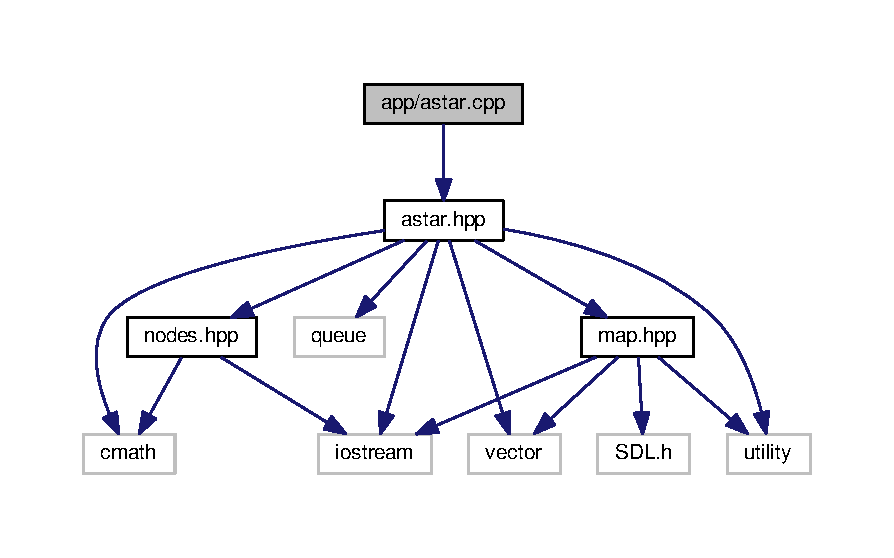
\includegraphics[width=350pt]{astar_8cpp__incl}
\end{center}
\end{figure}
\subsection*{Functions}
\begin{DoxyCompactItemize}
\item 
bool \hyperlink{astar_8cpp_acc59bcc4aa26b96977581ad5d6657457}{operator$>$} (const \hyperlink{classnodes}{nodes} \&node1, const \hyperlink{classnodes}{nodes} \&node2)
\end{DoxyCompactItemize}


\subsection{Detailed Description}
Definition of astar class methods. 

M\+IT License

Copyright (c) 2018 Yash Shah Permission is hereby granted, free of charge, to any person obtaining a copy of this software and associated documentation files (the \char`\"{}\+Software\char`\"{}), to deal in the Software without restriction, including without limitation the rights to use, copy, modify, merge, publish, distribute, sublicense, and/or sell copies of the Software, and to permit persons to whom the Software is furnished to do so, subject to the following conditions\+:

The above copyright notice and this permission notice shall be included in all copies or substantial portions of the Software.

T\+HE S\+O\+F\+T\+W\+A\+RE IS P\+R\+O\+V\+I\+D\+ED \char`\"{}\+A\+S I\+S\char`\"{}, W\+I\+T\+H\+O\+UT W\+A\+R\+R\+A\+N\+TY OF A\+NY K\+I\+ND, E\+X\+P\+R\+E\+SS OR I\+M\+P\+L\+I\+ED, I\+N\+C\+L\+U\+D\+I\+NG B\+UT N\+OT L\+I\+M\+I\+T\+ED TO T\+HE W\+A\+R\+R\+A\+N\+T\+I\+ES OF M\+E\+R\+C\+H\+A\+N\+T\+A\+B\+I\+L\+I\+TY, F\+I\+T\+N\+E\+SS F\+OR A P\+A\+R\+T\+I\+C\+U\+L\+AR P\+U\+R\+P\+O\+SE A\+ND N\+O\+N\+I\+N\+F\+R\+I\+N\+G\+E\+M\+E\+NT. IN NO E\+V\+E\+NT S\+H\+A\+LL T\+HE A\+U\+T\+H\+O\+RS OR C\+O\+P\+Y\+R\+I\+G\+HT H\+O\+L\+D\+E\+RS BE L\+I\+A\+B\+LE F\+OR A\+NY C\+L\+A\+IM, D\+A\+M\+A\+G\+ES OR O\+T\+H\+ER L\+I\+A\+B\+I\+L\+I\+TY, W\+H\+E\+T\+H\+ER IN AN A\+C\+T\+I\+ON OF C\+O\+N\+T\+R\+A\+CT, T\+O\+RT OR O\+T\+H\+E\+R\+W\+I\+SE, A\+R\+I\+S\+I\+NG F\+R\+OM, O\+UT OF OR IN C\+O\+N\+N\+E\+C\+T\+I\+ON W\+I\+TH T\+HE S\+O\+F\+T\+W\+A\+RE OR T\+HE U\+SE OR O\+T\+H\+ER D\+E\+A\+L\+I\+N\+GS IN T\+HE S\+O\+F\+T\+W\+A\+RE.

Yash Shah \begin{DoxyVersion}{Version}
1.\+0 This class defines the methods that finds optimum path given the map with obstacles. It also has a method that sorts the priority queue of nodes with ascending order of the cost function.
\end{DoxyVersion}
\begin{DoxyCopyright}{Copyright}
M\+IT License (c) 2018 
\end{DoxyCopyright}


\subsection{Function Documentation}
\index{astar.\+cpp@{astar.\+cpp}!operator$>$@{operator$>$}}
\index{operator$>$@{operator$>$}!astar.\+cpp@{astar.\+cpp}}
\subsubsection[{\texorpdfstring{operator$>$(const nodes \&node1, const nodes \&node2)}{operator>(const nodes &node1, const nodes &node2)}}]{\setlength{\rightskip}{0pt plus 5cm}bool operator$>$ (
\begin{DoxyParamCaption}
\item[{const {\bf nodes} \&}]{node1, }
\item[{const {\bf nodes} \&}]{node2}
\end{DoxyParamCaption}
)}\hypertarget{astar_8cpp_acc59bcc4aa26b96977581ad5d6657457}{}\label{astar_8cpp_acc59bcc4aa26b96977581ad5d6657457}
Gives priority to node with greater total cost to rearrange the priority Queue.


\begin{DoxyParams}{Parameters}
{\em p} & is a reference of a node \\
\hline
{\em q} & is a reference of a node\\
\hline
\end{DoxyParams}
\begin{DoxyReturn}{Returns}
true if the total cost (f cost) of p is greater, else false 
\end{DoxyReturn}

\hypertarget{main_8cpp}{}\section{app/main.cpp File Reference}
\label{main_8cpp}\index{app/main.\+cpp@{app/main.\+cpp}}


main cpp file for Project implementation  


{\ttfamily \#include $<$iostream$>$}\\*
{\ttfamily \#include $<$vector$>$}\\*
{\ttfamily \#include \char`\"{}astar.\+hpp\char`\"{}}\\*
{\ttfamily \#include \char`\"{}map.\+hpp\char`\"{}}\\*
{\ttfamily \#include \char`\"{}nodes.\+hpp\char`\"{}}\\*
Include dependency graph for main.\+cpp\+:
\nopagebreak
\begin{figure}[H]
\begin{center}
\leavevmode
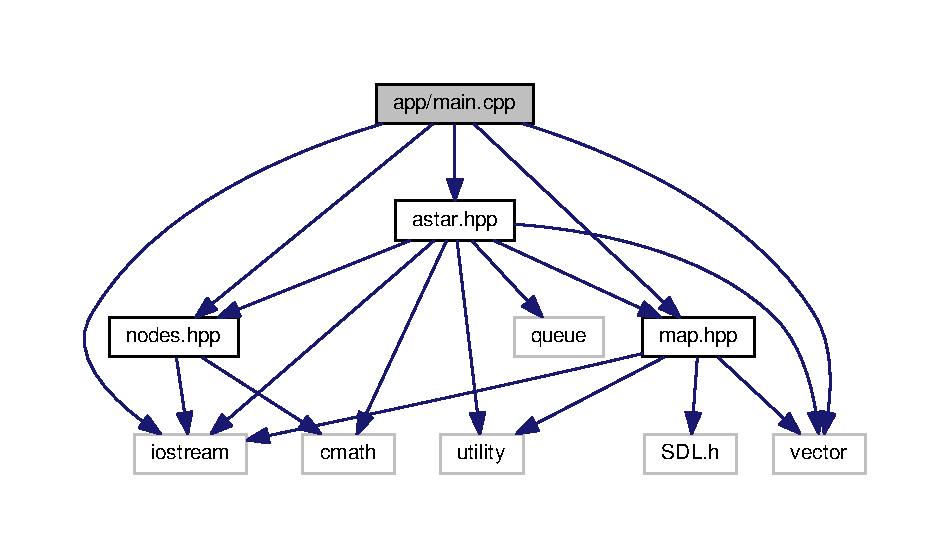
\includegraphics[width=350pt]{main_8cpp__incl}
\end{center}
\end{figure}
\subsection*{Functions}
\begin{DoxyCompactItemize}
\item 
int {\bfseries main} ()\hypertarget{main_8cpp_ae66f6b31b5ad750f1fe042a706a4e3d4}{}\label{main_8cpp_ae66f6b31b5ad750f1fe042a706a4e3d4}

\end{DoxyCompactItemize}


\subsection{Detailed Description}
main cpp file for Project implementation 

M\+IT License

Copyright (c) 2018 Yash Shah Permission is hereby granted, free of charge, to any person obtaining a copy of this software and associated documentation files (the \char`\"{}\+Software\char`\"{}), to deal in the Software without restriction, including without limitation the rights to use, copy, modify, merge, publish, distribute, sublicense, and/or sell copies of the Software, and to permit persons to whom the Software is furnished to do so, subject to the following conditions\+:

The above copyright notice and this permission notice shall be included in all copies or substantial portions of the Software.

T\+HE S\+O\+F\+T\+W\+A\+RE IS P\+R\+O\+V\+I\+D\+ED \char`\"{}\+A\+S I\+S\char`\"{}, W\+I\+T\+H\+O\+UT W\+A\+R\+R\+A\+N\+TY OF A\+NY K\+I\+ND, E\+X\+P\+R\+E\+SS OR I\+M\+P\+L\+I\+ED, I\+N\+C\+L\+U\+D\+I\+NG B\+UT N\+OT L\+I\+M\+I\+T\+ED TO T\+HE W\+A\+R\+R\+A\+N\+T\+I\+ES OF M\+E\+R\+C\+H\+A\+N\+T\+A\+B\+I\+L\+I\+TY, F\+I\+T\+N\+E\+SS F\+OR A P\+A\+R\+T\+I\+C\+U\+L\+AR P\+U\+R\+P\+O\+SE A\+ND N\+O\+N\+I\+N\+F\+R\+I\+N\+G\+E\+M\+E\+NT. IN NO E\+V\+E\+NT S\+H\+A\+LL T\+HE A\+U\+T\+H\+O\+RS OR C\+O\+P\+Y\+R\+I\+G\+HT H\+O\+L\+D\+E\+RS BE L\+I\+A\+B\+LE F\+OR A\+NY C\+L\+A\+IM, D\+A\+M\+A\+G\+ES OR O\+T\+H\+ER L\+I\+A\+B\+I\+L\+I\+TY, W\+H\+E\+T\+H\+ER IN AN A\+C\+T\+I\+ON OF C\+O\+N\+T\+R\+A\+CT, T\+O\+RT OR O\+T\+H\+E\+R\+W\+I\+SE, A\+R\+I\+S\+I\+NG F\+R\+OM, O\+UT OF OR IN C\+O\+N\+N\+E\+C\+T\+I\+ON W\+I\+TH T\+HE S\+O\+F\+T\+W\+A\+RE OR T\+HE U\+SE OR O\+T\+H\+ER D\+E\+A\+L\+I\+N\+GS IN T\+HE S\+O\+F\+T\+W\+A\+RE.

Yash Shah \begin{DoxyVersion}{Version}
1.\+0 This is the program to implement the A$\ast$ algorithm.
\end{DoxyVersion}
\begin{DoxyCopyright}{Copyright}
M\+IT License (c) 2018 
\end{DoxyCopyright}

\hypertarget{map_8cpp}{}\section{app/map.cpp File Reference}
\label{map_8cpp}\index{app/map.\+cpp@{app/map.\+cpp}}


Definition of map class methods.  


{\ttfamily \#include \char`\"{}map.\+hpp\char`\"{}}\\*
Include dependency graph for map.\+cpp\+:
\nopagebreak
\begin{figure}[H]
\begin{center}
\leavevmode
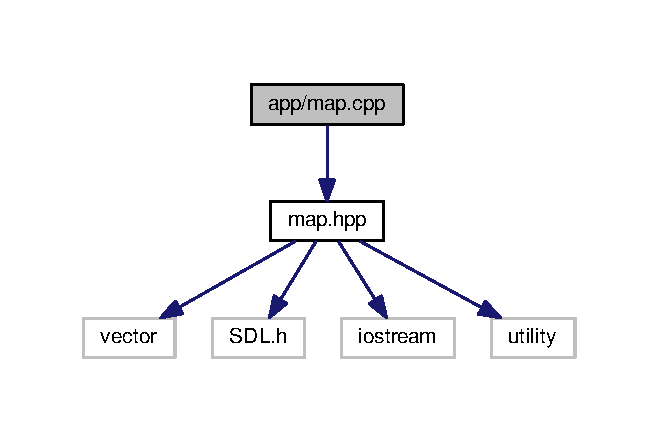
\includegraphics[width=316pt]{map_8cpp__incl}
\end{center}
\end{figure}


\subsection{Detailed Description}
Definition of map class methods. 

M\+IT License

Copyright (c) 2018 Yash Shah Permission is hereby granted, free of charge, to any person obtaining a copy of this software and associated documentation files (the \char`\"{}\+Software\char`\"{}), to deal in the Software without restriction, including without limitation the rights to use, copy, modify, merge, publish, distribute, sublicense, and/or sell copies of the Software, and to permit persons to whom the Software is furnished to do so, subject to the following conditions\+:

The above copyright notice and this permission notice shall be included in all copies or substantial portions of the Software.

T\+HE S\+O\+F\+T\+W\+A\+RE IS P\+R\+O\+V\+I\+D\+ED \char`\"{}\+A\+S I\+S\char`\"{}, W\+I\+T\+H\+O\+UT W\+A\+R\+R\+A\+N\+TY OF A\+NY K\+I\+ND, E\+X\+P\+R\+E\+SS OR I\+M\+P\+L\+I\+ED, I\+N\+C\+L\+U\+D\+I\+NG B\+UT N\+OT L\+I\+M\+I\+T\+ED TO T\+HE W\+A\+R\+R\+A\+N\+T\+I\+ES OF M\+E\+R\+C\+H\+A\+N\+T\+A\+B\+I\+L\+I\+TY, F\+I\+T\+N\+E\+SS F\+OR A P\+A\+R\+T\+I\+C\+U\+L\+AR P\+U\+R\+P\+O\+SE A\+ND N\+O\+N\+I\+N\+F\+R\+I\+N\+G\+E\+M\+E\+NT. IN NO E\+V\+E\+NT S\+H\+A\+LL T\+HE A\+U\+T\+H\+O\+RS OR C\+O\+P\+Y\+R\+I\+G\+HT H\+O\+L\+D\+E\+RS BE L\+I\+A\+B\+LE F\+OR A\+NY C\+L\+A\+IM, D\+A\+M\+A\+G\+ES OR O\+T\+H\+ER L\+I\+A\+B\+I\+L\+I\+TY, W\+H\+E\+T\+H\+ER IN AN A\+C\+T\+I\+ON OF C\+O\+N\+T\+R\+A\+CT, T\+O\+RT OR O\+T\+H\+E\+R\+W\+I\+SE, A\+R\+I\+S\+I\+NG F\+R\+OM, O\+UT OF OR IN C\+O\+N\+N\+E\+C\+T\+I\+ON W\+I\+TH T\+HE S\+O\+F\+T\+W\+A\+RE OR T\+HE U\+SE OR O\+T\+H\+ER D\+E\+A\+L\+I\+N\+GS IN T\+HE S\+O\+F\+T\+W\+A\+RE.

Yash Shah \begin{DoxyVersion}{Version}
1.\+0 This class implements the mapping of the algorithm. One method creates the map and other draws the path on the map.
\end{DoxyVersion}
\begin{DoxyCopyright}{Copyright}
M\+IT License (c) 2018 
\end{DoxyCopyright}

\hypertarget{nodes_8cpp}{}\section{app/nodes.cpp File Reference}
\label{nodes_8cpp}\index{app/nodes.\+cpp@{app/nodes.\+cpp}}


Definition of nodes class methods.  


{\ttfamily \#include \char`\"{}nodes.\+hpp\char`\"{}}\\*
Include dependency graph for nodes.\+cpp\+:
\nopagebreak
\begin{figure}[H]
\begin{center}
\leavevmode
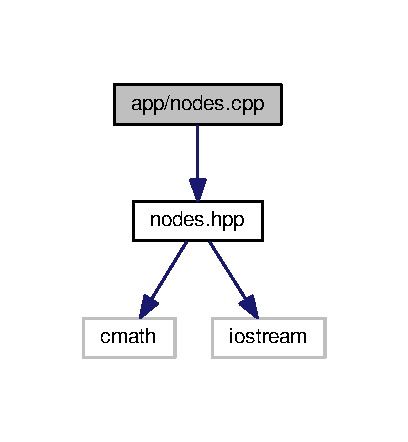
\includegraphics[width=196pt]{nodes_8cpp__incl}
\end{center}
\end{figure}


\subsection{Detailed Description}
Definition of nodes class methods. 

M\+IT License

Copyright (c) 2018 Yash Shah Permission is hereby granted, free of charge, to any person obtaining a copy of this software and associated documentation files (the \char`\"{}\+Software\char`\"{}), to deal in the Software without restriction, including without limitation the rights to use, copy, modify, merge, publish, distribute, sublicense, and/or sell copies of the Software, and to permit persons to whom the Software is furnished to do so, subject to the following conditions\+:

The above copyright notice and this permission notice shall be included in all copies or substantial portions of the Software.

T\+HE S\+O\+F\+T\+W\+A\+RE IS P\+R\+O\+V\+I\+D\+ED \char`\"{}\+A\+S I\+S\char`\"{}, W\+I\+T\+H\+O\+UT W\+A\+R\+R\+A\+N\+TY OF A\+NY K\+I\+ND, E\+X\+P\+R\+E\+SS OR I\+M\+P\+L\+I\+ED, I\+N\+C\+L\+U\+D\+I\+NG B\+UT N\+OT L\+I\+M\+I\+T\+ED TO T\+HE W\+A\+R\+R\+A\+N\+T\+I\+ES OF M\+E\+R\+C\+H\+A\+N\+T\+A\+B\+I\+L\+I\+TY, F\+I\+T\+N\+E\+SS F\+OR A P\+A\+R\+T\+I\+C\+U\+L\+AR P\+U\+R\+P\+O\+SE A\+ND N\+O\+N\+I\+N\+F\+R\+I\+N\+G\+E\+M\+E\+NT. IN NO E\+V\+E\+NT S\+H\+A\+LL T\+HE A\+U\+T\+H\+O\+RS OR C\+O\+P\+Y\+R\+I\+G\+HT H\+O\+L\+D\+E\+RS BE L\+I\+A\+B\+LE F\+OR A\+NY C\+L\+A\+IM, D\+A\+M\+A\+G\+ES OR O\+T\+H\+ER L\+I\+A\+B\+I\+L\+I\+TY, W\+H\+E\+T\+H\+ER IN AN A\+C\+T\+I\+ON OF C\+O\+N\+T\+R\+A\+CT, T\+O\+RT OR O\+T\+H\+E\+R\+W\+I\+SE, A\+R\+I\+S\+I\+NG F\+R\+OM, O\+UT OF OR IN C\+O\+N\+N\+E\+C\+T\+I\+ON W\+I\+TH T\+HE S\+O\+F\+T\+W\+A\+RE OR T\+HE U\+SE OR O\+T\+H\+ER D\+E\+A\+L\+I\+N\+GS IN T\+HE S\+O\+F\+T\+W\+A\+RE.

Yash Shah \begin{DoxyVersion}{Version}
1.\+0 This class creates the nodes and stores all the costs.
\end{DoxyVersion}
\begin{DoxyCopyright}{Copyright}
M\+IT License (c) 2018 
\end{DoxyCopyright}

\hypertarget{astar_8hpp}{}\section{include/astar.hpp File Reference}
\label{astar_8hpp}\index{include/astar.\+hpp@{include/astar.\+hpp}}


Header file for astar class.  


{\ttfamily \#include $<$iostream$>$}\\*
{\ttfamily \#include $<$cmath$>$}\\*
{\ttfamily \#include $<$queue$>$}\\*
{\ttfamily \#include $<$vector$>$}\\*
{\ttfamily \#include $<$utility$>$}\\*
{\ttfamily \#include \char`\"{}nodes.\+hpp\char`\"{}}\\*
{\ttfamily \#include \char`\"{}map.\+hpp\char`\"{}}\\*
Include dependency graph for astar.\+hpp\+:
\nopagebreak
\begin{figure}[H]
\begin{center}
\leavevmode
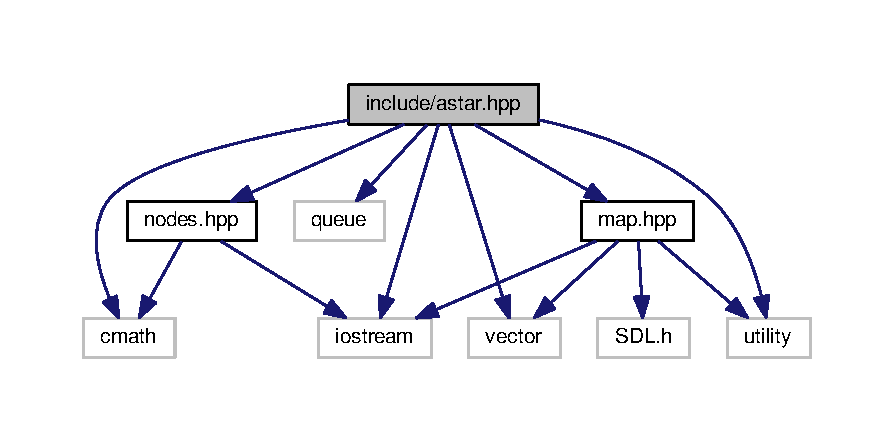
\includegraphics[width=350pt]{astar_8hpp__incl}
\end{center}
\end{figure}
This graph shows which files directly or indirectly include this file\+:
\nopagebreak
\begin{figure}[H]
\begin{center}
\leavevmode
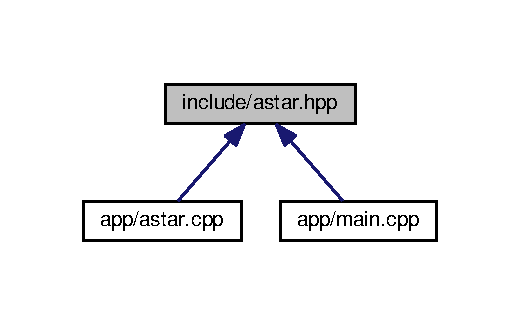
\includegraphics[width=250pt]{astar_8hpp__dep__incl}
\end{center}
\end{figure}
\subsection*{Classes}
\begin{DoxyCompactItemize}
\item 
class \hyperlink{classastar}{astar}
\end{DoxyCompactItemize}


\subsection{Detailed Description}
Header file for astar class. 

M\+IT License

Copyright (c) 2018 Yash Shah Permission is hereby granted, free of charge, to any person obtaining a copy of this software and associated documentation files (the \char`\"{}\+Software\char`\"{}), to deal in the Software without restriction, including without limitation the rights to use, copy, modify, merge, publish, distribute, sublicense, and/or sell copies of the Software, and to permit persons to whom the Software is furnished to do so, subject to the following conditions\+:

The above copyright notice and this permission notice shall be included in all copies or substantial portions of the Software.

T\+HE S\+O\+F\+T\+W\+A\+RE IS P\+R\+O\+V\+I\+D\+ED \char`\"{}\+A\+S I\+S\char`\"{}, W\+I\+T\+H\+O\+UT W\+A\+R\+R\+A\+N\+TY OF A\+NY K\+I\+ND, E\+X\+P\+R\+E\+SS OR I\+M\+P\+L\+I\+ED, I\+N\+C\+L\+U\+D\+I\+NG B\+UT N\+OT L\+I\+M\+I\+T\+ED TO T\+HE W\+A\+R\+R\+A\+N\+T\+I\+ES OF M\+E\+R\+C\+H\+A\+N\+T\+A\+B\+I\+L\+I\+TY, F\+I\+T\+N\+E\+SS F\+OR A P\+A\+R\+T\+I\+C\+U\+L\+AR P\+U\+R\+P\+O\+SE A\+ND N\+O\+N\+I\+N\+F\+R\+I\+N\+G\+E\+M\+E\+NT. IN NO E\+V\+E\+NT S\+H\+A\+LL T\+HE A\+U\+T\+H\+O\+RS OR C\+O\+P\+Y\+R\+I\+G\+HT H\+O\+L\+D\+E\+RS BE L\+I\+A\+B\+LE F\+OR A\+NY C\+L\+A\+IM, D\+A\+M\+A\+G\+ES OR O\+T\+H\+ER L\+I\+A\+B\+I\+L\+I\+TY, W\+H\+E\+T\+H\+ER IN AN A\+C\+T\+I\+ON OF C\+O\+N\+T\+R\+A\+CT, T\+O\+RT OR O\+T\+H\+E\+R\+W\+I\+SE, A\+R\+I\+S\+I\+NG F\+R\+OM, O\+UT OF OR IN C\+O\+N\+N\+E\+C\+T\+I\+ON W\+I\+TH T\+HE S\+O\+F\+T\+W\+A\+RE OR T\+HE U\+SE OR O\+T\+H\+ER D\+E\+A\+L\+I\+N\+GS IN T\+HE S\+O\+F\+T\+W\+A\+RE.

Yash Shah \begin{DoxyVersion}{Version}
1.\+0 This class defines the methods that finds optimum path given the map with obstacles. It also has a method that sorts the priority queue of nodes with ascending order of the cost function.
\end{DoxyVersion}
\begin{DoxyCopyright}{Copyright}
M\+IT License (c) 2018 
\end{DoxyCopyright}

\hypertarget{map_8hpp}{}\section{include/map.hpp File Reference}
\label{map_8hpp}\index{include/map.\+hpp@{include/map.\+hpp}}


Header file for map class.  


{\ttfamily \#include $<$vector$>$}\\*
{\ttfamily \#include $<$S\+D\+L.\+h$>$}\\*
{\ttfamily \#include $<$iostream$>$}\\*
{\ttfamily \#include $<$utility$>$}\\*
Include dependency graph for map.\+hpp\+:
\nopagebreak
\begin{figure}[H]
\begin{center}
\leavevmode
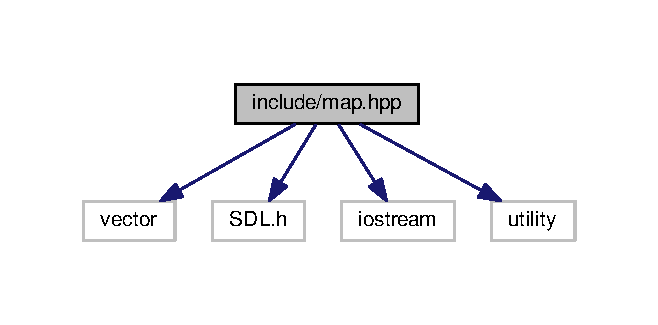
\includegraphics[width=316pt]{map_8hpp__incl}
\end{center}
\end{figure}
This graph shows which files directly or indirectly include this file\+:
\nopagebreak
\begin{figure}[H]
\begin{center}
\leavevmode
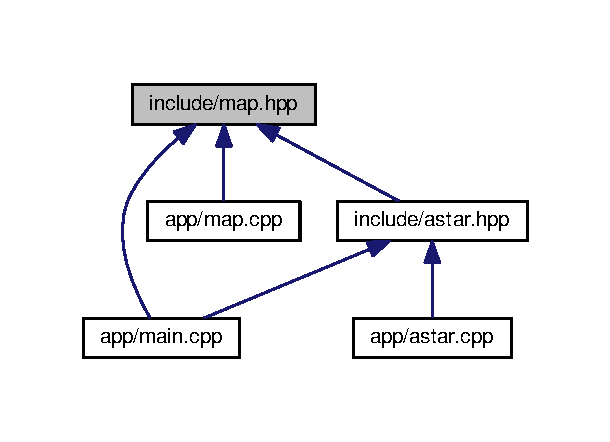
\includegraphics[width=293pt]{map_8hpp__dep__incl}
\end{center}
\end{figure}
\subsection*{Classes}
\begin{DoxyCompactItemize}
\item 
class \hyperlink{classmap}{map}
\end{DoxyCompactItemize}


\subsection{Detailed Description}
Header file for map class. 

M\+IT License

Copyright (c) 2018 Yash Shah Permission is hereby granted, free of charge, to any person obtaining a copy of this software and associated documentation files (the \char`\"{}\+Software\char`\"{}), to deal in the Software without restriction, including without limitation the rights to use, copy, modify, merge, publish, distribute, sublicense, and/or sell copies of the Software, and to permit persons to whom the Software is furnished to do so, subject to the following conditions\+:

The above copyright notice and this permission notice shall be included in all copies or substantial portions of the Software.

T\+HE S\+O\+F\+T\+W\+A\+RE IS P\+R\+O\+V\+I\+D\+ED \char`\"{}\+A\+S I\+S\char`\"{}, W\+I\+T\+H\+O\+UT W\+A\+R\+R\+A\+N\+TY OF A\+NY K\+I\+ND, E\+X\+P\+R\+E\+SS OR I\+M\+P\+L\+I\+ED, I\+N\+C\+L\+U\+D\+I\+NG B\+UT N\+OT L\+I\+M\+I\+T\+ED TO T\+HE W\+A\+R\+R\+A\+N\+T\+I\+ES OF M\+E\+R\+C\+H\+A\+N\+T\+A\+B\+I\+L\+I\+TY, F\+I\+T\+N\+E\+SS F\+OR A P\+A\+R\+T\+I\+C\+U\+L\+AR P\+U\+R\+P\+O\+SE A\+ND N\+O\+N\+I\+N\+F\+R\+I\+N\+G\+E\+M\+E\+NT. IN NO E\+V\+E\+NT S\+H\+A\+LL T\+HE A\+U\+T\+H\+O\+RS OR C\+O\+P\+Y\+R\+I\+G\+HT H\+O\+L\+D\+E\+RS BE L\+I\+A\+B\+LE F\+OR A\+NY C\+L\+A\+IM, D\+A\+M\+A\+G\+ES OR O\+T\+H\+ER L\+I\+A\+B\+I\+L\+I\+TY, W\+H\+E\+T\+H\+ER IN AN A\+C\+T\+I\+ON OF C\+O\+N\+T\+R\+A\+CT, T\+O\+RT OR O\+T\+H\+E\+R\+W\+I\+SE, A\+R\+I\+S\+I\+NG F\+R\+OM, O\+UT OF OR IN C\+O\+N\+N\+E\+C\+T\+I\+ON W\+I\+TH T\+HE S\+O\+F\+T\+W\+A\+RE OR T\+HE U\+SE OR O\+T\+H\+ER D\+E\+A\+L\+I\+N\+GS IN T\+HE S\+O\+F\+T\+W\+A\+RE.

Yash Shah \begin{DoxyVersion}{Version}
1.\+0 This class implements the mapping of the algorithm. One method creates the map and other draws the path on the map.
\end{DoxyVersion}
\begin{DoxyCopyright}{Copyright}
M\+IT License (c) 2018 
\end{DoxyCopyright}

\hypertarget{nodes_8hpp}{}\section{include/nodes.hpp File Reference}
\label{nodes_8hpp}\index{include/nodes.\+hpp@{include/nodes.\+hpp}}


Header file for nodes class.  


{\ttfamily \#include $<$cmath$>$}\\*
{\ttfamily \#include $<$iostream$>$}\\*
Include dependency graph for nodes.\+hpp\+:
\nopagebreak
\begin{figure}[H]
\begin{center}
\leavevmode
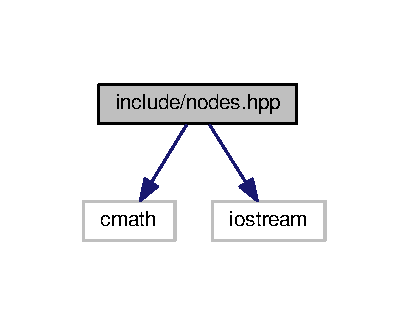
\includegraphics[width=196pt]{nodes_8hpp__incl}
\end{center}
\end{figure}
This graph shows which files directly or indirectly include this file\+:
\nopagebreak
\begin{figure}[H]
\begin{center}
\leavevmode
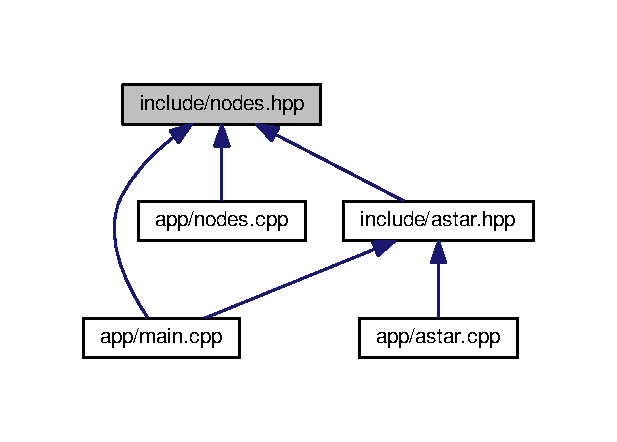
\includegraphics[width=296pt]{nodes_8hpp__dep__incl}
\end{center}
\end{figure}
\subsection*{Classes}
\begin{DoxyCompactItemize}
\item 
class \hyperlink{classnodes}{nodes}
\end{DoxyCompactItemize}


\subsection{Detailed Description}
Header file for nodes class. 

M\+IT License

Copyright (c) 2018 Yash Shah Permission is hereby granted, free of charge, to any person obtaining a copy of this software and associated documentation files (the \char`\"{}\+Software\char`\"{}), to deal in the Software without restriction, including without limitation the rights to use, copy, modify, merge, publish, distribute, sublicense, and/or sell copies of the Software, and to permit persons to whom the Software is furnished to do so, subject to the following conditions\+:

The above copyright notice and this permission notice shall be included in all copies or substantial portions of the Software.

T\+HE S\+O\+F\+T\+W\+A\+RE IS P\+R\+O\+V\+I\+D\+ED \char`\"{}\+A\+S I\+S\char`\"{}, W\+I\+T\+H\+O\+UT W\+A\+R\+R\+A\+N\+TY OF A\+NY K\+I\+ND, E\+X\+P\+R\+E\+SS OR I\+M\+P\+L\+I\+ED, I\+N\+C\+L\+U\+D\+I\+NG B\+UT N\+OT L\+I\+M\+I\+T\+ED TO T\+HE W\+A\+R\+R\+A\+N\+T\+I\+ES OF M\+E\+R\+C\+H\+A\+N\+T\+A\+B\+I\+L\+I\+TY, F\+I\+T\+N\+E\+SS F\+OR A P\+A\+R\+T\+I\+C\+U\+L\+AR P\+U\+R\+P\+O\+SE A\+ND N\+O\+N\+I\+N\+F\+R\+I\+N\+G\+E\+M\+E\+NT. IN NO E\+V\+E\+NT S\+H\+A\+LL T\+HE A\+U\+T\+H\+O\+RS OR C\+O\+P\+Y\+R\+I\+G\+HT H\+O\+L\+D\+E\+RS BE L\+I\+A\+B\+LE F\+OR A\+NY C\+L\+A\+IM, D\+A\+M\+A\+G\+ES OR O\+T\+H\+ER L\+I\+A\+B\+I\+L\+I\+TY, W\+H\+E\+T\+H\+ER IN AN A\+C\+T\+I\+ON OF C\+O\+N\+T\+R\+A\+CT, T\+O\+RT OR O\+T\+H\+E\+R\+W\+I\+SE, A\+R\+I\+S\+I\+NG F\+R\+OM, O\+UT OF OR IN C\+O\+N\+N\+E\+C\+T\+I\+ON W\+I\+TH T\+HE S\+O\+F\+T\+W\+A\+RE OR T\+HE U\+SE OR O\+T\+H\+ER D\+E\+A\+L\+I\+N\+GS IN T\+HE S\+O\+F\+T\+W\+A\+RE.

Yash Shah \begin{DoxyVersion}{Version}
1.\+0 This class creates the nodes and stores all the costs.
\end{DoxyVersion}
\begin{DoxyCopyright}{Copyright}
M\+IT License (c) 2018 
\end{DoxyCopyright}

%--- End generated contents ---

% Index
\backmatter
\newpage
\phantomsection
\clearemptydoublepage
\addcontentsline{toc}{chapter}{Index}
\printindex

\end{document}
